\documentclass{article}
\usepackage{graphicx}
\title{My First \LaTeX{} Document}
\author{Zhou Lvwen}
\date{\today} 


\begin{document}
\maketitle
\begin{abstract}
Short introduction to subject of the paper. 
\end{abstract}

% ------------------------------------------------------
\section{Introduction}
Make it possible for all to write documents with \LaTeX{}!

% ------------------------------------------------------
\section{List}
\LaTeX{} can compose many documents, including but not limited to the following document types: 
\begin{itemize}
\item article
\item book 
\item report 
\item letter 
\end{itemize}

% ------------------------------------------------------
\section{Math}
Math in text is called in line math just put \$ character around 
the math think. Like $a^2 + b^2 = c^2$. It looks better if you use this 
\[a^2 + b^2 = c^2\]

% ------------------------------------------------------
\section{Tabular}
\begin{tabular}{|l|c|r|}
\hline
first column & second column & third column\\
\hline 
l stand for left & c for center & r for right\\
\hline 
\end{tabular} 

% ------------------------------------------------------
\section{Figure}
It's easy to insert a figure. 
\begin{figure}
  \centering
  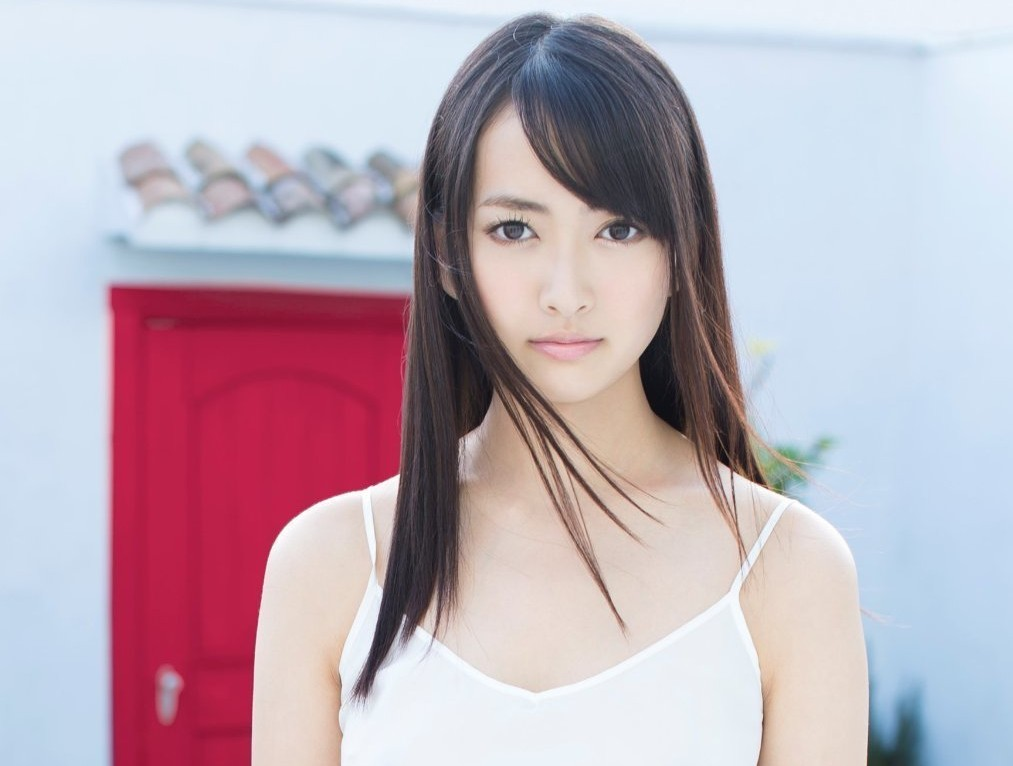
\includegraphics[scale=0.2]{Risa.jpg}
  \caption{A simple girl.}
  \label{fig:birds}
\end{figure}

% ------------------------------------------------------
\section{Citation}\label{conclusions}
There is no longer \LaTeX{} example which was written by \cite{zhou2018latex}.

\begin{thebibliography}{9}
\bibitem{zhou2018latex} Zhou Lvwen. First and last \LaTeX{} example, 2018.
\end{thebibliography}

\end{document}

